\documentclass[usenatbib,fleqn]{mnras}

\makeatletter
\newlength{\abovecaptionskip}%
\setlength{\abovecaptionskip}{10\p@}
\makeatother


\usepackage{threeparttable}
 

\usepackage{amsmath,amssymb}
\usepackage{mathrsfs}
\usepackage{graphicx}
\usepackage{epstopdf}
%\usepackage{hyperref}
\epstopdfsetup{outdir=./figures/}
\graphicspath{{./figures/}}
\usepackage{url}
%\usepackage{aas_macros}

\newcommand\lsim{\mathrel{\rlap{\lower4pt\hbox{\hskip1pt$\sim$}}
    \raise1pt\hbox{$<$}}}
\newcommand\gsim{\mathrel{\rlap{\lower4pt\hbox{\hskip1pt$\sim$}}
    \raise1pt\hbox{$>$}}}


\newcommand       \be          {\begin{eqnarray}}
\newcommand       \ee          {\end{eqnarray}}
\newcommand{\Mbh}[1][]{M_{\bullet#1}}
\newcommand{\Menc}{M_{\rm enc}}
\renewcommand{\th}{t_h}
\newcommand{\Msun}{{\rm M_\odot}}
\newcommand{\pyear}{{\rm yr}^{-1}}

% write title (with email and institute)
\title{TDE jets}

\begin{document}

\begin{abstract}
  Radio light curves calculated for TDE jets. CNM
  densities based on \citet{Generozov+2015}. 
\end{abstract}
\section{Introduction}
\label{sec:intro}
When a star in a galactic nucleus is deflected too close to the
central supermassive black hole (BH), it can be torn apart by tidal
forces.  During this tidal disruption event (TDE), roughly half of the
stellar debris remains bound to the BH, while the other half is flung
outwards and unbound from the system.  The bound material, following a
potentially complex process of debris circularization
(\citealt{Guillochon&RamirezRuiz13},\citealt{Hayasaki+13},\citealt{Hayasaki+15},\citealt{Shiokawa+15},\citealt{Bonnerot+15}),
accretes onto the BH, creating a luminous flare lasting months to
years \citep{Hills1975, Carter+1982, Rees1988}.

Many thermal TDE flares have now been identified at UV/optical
\citep{van-Velzen+2011, Gezari+2012, Chornock+2014, Arcavi+2014} and
soft x-ray wavelengths \citep{Esquej+2007}.  Beginning with the
discovery of {\it Swift} J1644+57 in 2011, three additional TDEs have
been discovered by their non-thermal x-ray emission
(\citealt{Bloom+2011, Levan+11, Burrows+11, Zauderer+2011, Cenko+2012,
  Pasham+15, Brown+2015}).  Unlike the thermal TDEs, these events are
the result of emission from a transient relativistic jet beamed along
our line of sight, similar to the blazar geometry of active galactic
nuclei (AGN).  In addition to their highly variable X-ray emission,
which likely originates from the base of the jet, these events are
characterized by radio synchrotron emission.  The latter, more slowly
evolving, is powered by shocks formed at the interface between the jet
and surrounding circumnuclear medium (CNM)
(\citealt{Giannios&Metzger11,Metzger+12}), analagous to the afterglow
of a gamma-ray burst.

Although a handful of jetted TDE flares have been observed, their
volumetric rate is a very small fraction $\sim 10^{-4}$ of the rate of
the observed thermal TDE flares (e.g., \citealt{Burrows+11}), and an
even smaller fraction of the theoretically predicted TDE rate
(\citealt{Stone&Metzger15}).  One potential explanation for this
discrepency is that the majority of TDEs produce powerful jets, but
their non-thermal X-ray emission is relativistically beamed into a
small angle $\theta_{\rm b}$, making them visible to only a small
fraction of observers.  However, in order to explain the required
beaming fraction $f_b \approx \theta_{b}^{2}/2 \sim 10^{-4}$ would
require $\theta_{\rm b} \sim 0.01$ and hence a jet with a bulk Lorentz
factor of $\Gamma \gtrsim 1/\theta_j \sim 100$, much higher than
typically inferred for AGN jets or inferred for {\it Swift} J1644+57
(\citealt{Metzger+12}).

The low detection rate of non-thermal TDE may instead indicate that
jets are intrinsically rare in TDEs, or the conditions of the
surrounding environment are unfavorable for producing bright emission.
Jets could be rare if they require, for instance, a highly
super-Eddington accretion rate (\citealt{DeColle+12}), a TDE from a
deeply plunging stellar orbit (\citealt{Metzger&Stone15}), or a
particularly strong magnetic flux threading the star
(\citealt{Tchekhovskoy+14,Kelley+14}).  Alternatively, jet formation
or its X-ray emission could be suppressed if the disk undergoes
Lens-Thirring precession due to a misalignment between the angular
momentum of the BH and that of the disrupted star
(\citealt{Stone&Loeb12}).  In the latter case, however, even a `messy'
jet could still be produced, which produces luminous non-thermal radio
synchrotron emission as it interacts the surrounding CNM.  The radio
emission from an off-axis is predicted to be relatively isotropic
(\citealt{Giannios&Metzger11},\citealt{Mimica+15}).

Observational campaigns have been conducted to follow-up thermal TDE
flares at radio wavelengths on timescales of months to decades after
the outburst (\citealt{Bower+13}; \citealt{van-Velzen+2013}; see Table
1 of \cite{Mimica+15} for a compilation).  \citet{van-Velzen+2013}
detected no radio emission from their 7 candidates, while
\citet{Bower+13} detected radio emission from two out of ROSAT flares:
RX J1420.4+5334 and IC 3599.  However, for RX J1420.4+5334 the radio
emission was observed in a different galaxy than that originally
identified by \citet{Komossa&Greiner99} as the host.  Furthermore, the
highly irregular behavior of IC 3599, including multiple outbursts
over the past few decades from this low luminosity AGN
(e.g.~\citealt{Campana+15}), calls into question whether this event is
a true TDE at all.  \citet{Bower+13} and \citet{van-Velzen+2013} use a
simple model for the radio emission as a Sedov blastwave, to conclude
that $\lesssim 10\%$ of TDEs produce jetted TDE emission at a level
similar to that produced in {\it Swift} J1644+57.  \citet{Mimica+15}
used 2D hydrodynamical models, coupled with a synchrotron radiation
transport calculation, to model the on-axis emission from {\it Swift}
J1644+57, which they then extended to the case of an off-axis viewing
angle to conclude that most previous TDEs should have been detected if
their jets were as powerful.

Previous works (\citet{Bower+13}; \citet{van-Velzen+2013};
\citealt{Mimica+15}) have generally assumed that all TDEs occur in a
similar environment as {\it Swift} J1644+57.  However, in general the
gas density in a galactic nucleus depends sensitively on the sources
of gas from stellar winds, and the sources of gas heating
(\citealt{Quataert04},\citealt{Generozov+2015}).  In a gamma-ray
burst, the environment the jet emerges is relatively well-understood
to be the wind of the massive progenitor star, or the ISM of the host
galaxy.  However, in a TDE, the density could in principle be orders
of magnitude higher.

In this paper we address the range of gas densities encountered by
jetted TDEs and estimate their synchrotron emission by means of
analytic calculations and numerical simulations.  If we are led to the
conclusion that the observable radio emission should be detected for
all allowed CNM densities, then we are lead to the conclusion that
most TDEs do not launch J1644-like jets.  This result would have
significant implications for the physics of jet launching in TDEs and
more broadly.

In $\S\ref{sec:cnm}$ we explore the expected CNM densities using the
formalism developed in \citet{Generozov+2015} (hereafter GSM15) to
calculate the CNM profile for different assumptions about the stellar
population in the galactic nucleus.  A younger stellar population
produces significant wind mass loss from O \& B stars. In contrast,
the rate of wind mass loss from an older population, which lacks these
massive stars, could $\sim 2$ orders of magnitude smaller.  We show
that the requirement of a physical stellar population, combined with
condition of thermal stability of the hot gas phase, limits the gas
density on a scale of $10^{18}$ cm to a range of $n_{18} \sim
0.1-10^{3}$ cm$^{-3}$.  Although these limits come from considering
only the hot phase of gas, we show empirically based on the measured
distribution of Eddington ratios that the average density in most
galactic nuclei is bracketed by this range {\bf AG rephrased}.

As a second component of this paper, in In $\S\ref{sec:jet}$ we
explore the expected synchrotron emission from J1644+57-like across
the allowed range of CNM conditions.  We start in
$\S\ref{sec:analytic}$ with analytic conditions.  Then in
$\S\ref{sec:numerical}$ use both 1d and 2d hydrodynamic models to
simulate the jet propagating through the CNM and compare the results
in $\S\ref{sec:2d}$. In $\S\ref{sec:results}$ we show radio
light-curves from our 1d models for a wide range of CNM densities, to
illustrate qualitatively how much varying the CNM density by itself
could change the radio light-curve.  We discuss the implications of
our models for detections of TDEs by future radio surveys in
$\S\ref{sec:disc}$, and summarize our conclusions in
$\S\ref{sec:conc}$.

\section{Range of CNM Densities}
\label{sec:cnm}

In this section we place theoretical and observational constraints on the radial profile of the gas density $n(r)$ in the nuclei of galaxies, which is typically takes on a power-law form $n = n_{18}(r/10^{18}{\rm cm})^{-\gamma}$ with $\gamma \approx 1-1.5$.  We focus constraining the normalization $n_{18}$ of the density at $r = 10^{18}$ cm, as the latter represents the approximate deceleration radius of the blast wave ($\S\ref{sec:analytic}$) 

\subsection{Analytic Constraints on CNM Density}

\subsubsection{CNM Model}

The dominant source of gas injection into the CNM of quiescent
galaxies is winds from stars in the galactic nucleus. The 1D spherical
hydrodynamic equations with stellar wind mass injection are
(e.g. \citealt{Holzer+1970}; \citealt{Quataert04}) 
\begin{align}
  &\frac{\partial \rho}{\partial t}+\frac{1}{r^2}\frac{\partial}{\partial r}\left(\rho r^2 v\right)=q \label{eq:drhodt}\\
  &\rho \left(\frac{\partial v}{\partial t} + v\frac{\partial
      v}{\partial r}\right) =-\frac{\partial p}{\partial r}- \rho\frac{GM_{\rm enc}}{r^{2}} -q v \label{eq:dvdt}\\
  &\rho T\left(\frac{\partial s}{\partial t} + v\frac{\partial
      s}{\partial
      r}\right)=q\left[\frac{v^2}{2}+\frac{v_w^2}{2}-\frac{\gamma}{\gamma-1}
    \frac{p}{\rho} \right] ,
\label{eq:dsdt}
\end{align}
where $\rho = \mu m_p n$, $v$, $p$, and $s$ are the density, velocity, pressure (assumed to be an ideal gas with $\mu = 0.62$), and
specific entropy, respectively.  The enclosed mass $\Menc = M_{\bullet} + M_{\star}$ includes both the black hole mass $M_{\bullet}$ and enclosed stellar mass $M_{\star} \propto \int \rho_{\star}r^{2}dr$.  

The mass source term $q =\eta \rho_\star/\th$ is the mass injection
rate per unit volume per unit time, where $\rho_\star$ is the stellar
density.  At small radii of interest, inside the Nuker `break' radius,
the stellar density follows $\rho_\star\sim r^{-\delta_1}$, where
$\delta_1 = 0-1$ is the inner Nuker profile \citep{Lauer+2007}.  The energy
source term $\propto v_w^{2}$ parameterizes the heating rate of the
gas, as physically results from stellar wind kinetic energy,
supernovae, and black hole feedback.

For a cusp galaxy ($\delta_1> 0.5$), \citet{Generozov+2015} show that the gas density obeys $n \sim
r^{-1}$, with a normalization
\begin{equation}
n_{18}\simeq 0.4 \Mbh[,7]^{0.5} \eta_{0.02} v_{500}^{-1.5} {\rm
  cm^{-3}},
\label{eq:n18}
\end{equation}
where $\Mbh[,7]= \Mbh/10^7 \Msun$,
$\eta_{0.02}= \eta/0.02$, and $v_{500}=v_w/500$ km s$^{-1}$, and we have assumed a fixed slope for the stellar density
power law slope $\delta_1=1.8$. 

Equation (\ref{eq:n18}) shows that the gas density is sensitive to the
mass return parameter and the heating rate, which are related to the
star formation history. Young, massive stars put out very energetic
winds with $v_w\simeq 1000$ km s$^{-1}$ with a high mass return rate,
$\eta\simeq 100$.  In contrast, stars with age comparable to that of
the universe will have slow winds with speeds of order\footnote{In the
  case of such low heating, $v_w \lesssim \sigma$, the heating of the
  gas is dominated by the velocity dispersion of the nucleus
  $\sigma$.} $\sim 10$ km s$^{-1}$ and mass return parameters,
$\eta\simeq0.02$. In the next section we explore the range of mass
return parameters, heating rates, and gas densities allowed by
plausible star formation histories.

\subsubsection{Allowed Density Range for Thermal Stability}

Equation (\ref{eq:n18}) shows that increasing the mass return
parameter, $\eta$, or decreasing the heating parameter $v_w$,
increases the gas density, $n_{18}$.  However, as we now show, one
cannot increase the $\eta$ or decrease $v_w$ indefinitely, as the CNM
will become thermally unstable.  Defining thermally instability as
occuring when the cooling time of the gas is less than 10 times the
local dynamical timescale (\citealt{McCourt+2012}), GSM15 show that the
CNM is thermally unstable for wind heating rates below a critical
value
\begin{equation}
v_{\rm w,TI}\simeq 200 \eta_{0.02}^{0.17} \Mbh[,7]^{0.08} \,{\rm km \,\,s^{-1}},
\label{eq:ti}
\end{equation}
where we have assumed line cooling dominates free-free emission, as is valid for $v_{\rm w} \lesssim 10^{3}$ km s$^{-1}$.

If the hot phase of CNM reaches a thermally unstable condition
($v_{\rm w} \lesssim v_{\rm w,TI}$), it is likely that portions of the
hot phase will condense into cold gas, eventually resulting in star
formation.  Therefore, it is reasonable to hypothesize that the CNM
will regulate itself to the condition $v_w \lesssim v_{\rm w,TI}$ (a
similar argument has been made on larger scales in galaxies;
\citealt{Voit+2015}).  The condition places an upper limit on the gas
density
\begin{equation}
n_{18} \lesssim n_{\rm 18,TI}\simeq 1.6 \eta_{0.02}^{0.75} \Mbh[,7]^{0.38} \, {\rm cm^{-3}}\,\,\,\text{Thermal Stability}
\label{eq:n18ti},
\end{equation}
where we have used equations~\eqref{eq:n18} and~\eqref{eq:ti}.

The maximum physical value of $\eta\simeq 400$ occurs $\sim 3$ Myr after a burst of star formation.\footnote{For details
  of how to calculate $\eta$ for a given star formation history see
  appendix C of \citet{Generozov+2015}.}  Evaluating equation~\eqref{eq:n18ti} with
$\eta=400$ gives the maximum thermally-stable CNM density
\begin{equation}
n_{\rm 18,max} \simeq 2.7\times 10^{3} \Mbh[,7]^{0.38} {\rm cm^{-3}}
\label{eq:n18max}
\end{equation}

Although such a large gas density would be present in the immediate aftermath of a starburst, the wind mass loss rate (and hence the gas density) declines as $\eta \sim t^{-3}$. Thus we expect the gas density would decline by an order of magnitude after a few Myr. Note that type II Supernovae could inject additional mass into the CNM, but this injection would be intermittent (e.g. the time between SNe would be long compared to a dynamical time).

% {\bf AG the subsequent discussion relies on out of date parameters for
% the stellar light profile for NGC 3156. In calculating the profile, we
% assume it turns over at 2 pc. In reality it probably turns over at ~20
% pc, and becomes a typical cusp profile. Next few paragraphs should be axed.}
% However, we also find high gas densities ($n_{18}\sim 2000$ cm$^{-3}$)
% may be present for E+A galaxies with stellar ages $\tau_\star\sim
% 10^8-10^9$ years. Although E+A galaxies are rare they host $\sim 20
% \%$ of all optically selected TDE candidates. Thus, the high density
% limit could be relevant for a sizable fraction of TDEs {\bf AG citation
%   needed here...}

% {\bf AG too much detail?} We construct a gas density profile for the
% nearby E+A galaxy NGC 3156. This galaxy has a stellar light profile
% measured with high resolution HST photometry. \citealt{Krajnovic+2013}
% find a steep inner stellar density profile with $\rho_\star\sim
% r^{-2.78}$, albeit with a possible turnover to a shallower profile at
% $r \sim 2-4$ pc. We assume a core-like profile with $\rho_\star \sim
% r^{-1.1}$ for $r<2$ pc.

% We find a thermally stable profile for NGC 3156 for mass
% return parameter $\eta\simeq0.5$ and Type Ia supernova heating
% $v_w\simeq600 $ km/s, as expected for 1 Gyr after a burst of star
% formation. We find $n \sim 2000 (r/10^{18} {\rm cm})^{-1.3}$
% cm$^{-3}$, for $r<2$ pc, $n\sim r^{-2}$ for $r>2$ pc, which is quite
% similar to the profile for a normal cusp galaxy with break at $r_b$=2
% pc. {\bf AG--w/o turnover the inner density slope would be -2--possibly
% do a special case?}

% Such a large gas density should produce a large x-ray luminosity in
% the galactic nucleus from metal line cooling and free-free emission.
% In particular our model for the E+A galaxy predicts an x-ray
% luminosity of $\sim$ few $\times 10^{39}$ egs/s, from the inner few
% parsecs of the galaxy {\bf AG--reran with proper normalization of the
%   cooling function (this was incorrect in GSM15). Would be good to
%   double-check these results.}


% {\bf AG--we could probably look for archival ROSAT observations for
%   non-active galaxies, to constrain the gas densities
%   there. For any galaxy w/o central x-ray source could put upper
%   limits on the gas density based on the free-free emission we would
%   have to have.}
% We found an archival X-ray observation from ROSAT for this galaxy {\bf
%   AG describe observation here; look for other observation}. There are
% no X-ray sources consistent with the galactic nucleus, which gives a
% 90\% confidence of upper limit $<2.4$ counts over the $\sim$400 s
% exposure time. We then use this non-detection to put an upper limit on
% the unresolved x-ray flux from the galactic nucleus using the
% web-PIMMS
% tool\footnote{https://heasarc.gsfc.nasa.gov/cgi-bin/Tools/w3pimms/w3pimms.pl}. We
% use an APEC emission model, temperature of ($10^{7} K$--the
% approximate temperature of the gas for radii dominating the x-ray
% emission a solar metallicity ({\bf AG Check for metallicity
%   measurements for this galaxy}), and $2.43\times 10^{20} {\rm
%   cm^{-2}}$ for the galactic HI column density\footnote{from
%   https://heasarc.gsfc.nasa.gov/cgi-bin/Tools/w3nh/w3nh.pl}. With
% these parameters non-detection gives an upper limit on the flux of
% $\lsim 2\times 10^{39}$ ergs/s {\bf AG check for other x-ray
%   images}. Thus, the non-detection is marginally consistent with the
% model, though it shows the density cannot be much higher than we
% predict.

What is the smallest plausible CNM density? This would correspond to a
small mass return parameter and a high heating rate. The mass return
parameter, $\eta=0.02$, reaches its minimum value for a stellar
population that is a Hubble time old. A stellar population
that is $<$ 3 Myr old will have a heating rate, $v_w=3,000$ km s$^{-1}$.

A stellar population in which a small fraction, $f$ of the stars
formed $\lsim 3$ Myr ago and the rest are a Hubble time old, will have
both a high heating rate and a low mass return rate. In this scenario
$n_{18}$ will be minimized for $f=4\times 10^{-4}$. Both old and young
stars contribute significantly to the mass injection rate giving
$\eta\simeq 0.03$, while the young star dominate the heating
$v_w\simeq 3,000$ km/s and thermally stabilize the gas. These
parameters provide the minimum possible CNM gas density
\begin{equation}
n_{\rm 18,min}\simeq 0.06 \Mbh[,7]^{0.5} {\rm cm^{-3}}
\label{eq:n18min}
\end{equation}

We illustrate how the mass return parameter, heating rate, and
density vary with star formation history in Fig.~\ref{fig:param}. The
gray lines represent a two-burst model for star formation in which a
fraction, $f$, of the stars formed $<$ 3 Myr ago and the remainder
formed a Hubble time ago (top gray line) or 1 Gyr ago (bottom red
line).  Towards the top right the $f=1$ and the young stars dominate
the mass injection rate and the heating rate.  Moving towards the
left, $f$ decreases, along with the mass return rate, and density
(blue lines), but the heating rate, $v_w$, remains $\gsim 1000$ km/s
except for very small values of $f$. The bend in the top, solid, gray curve
corresponds to the minimum possible CNM density.

The dashed, gray line also represents a two burst formation history
but the older burst is $\sim 3$ Myr old (right at the age when stars
are beginning to leave the main sequence, increasing the mass
injection rate. Towards the lower right of the dashed, gray line these
somewhat older stars dominate the mass injection into the CNM,
increasing the density past the thermal instability threshold (thick,
black line). The intersection between the dashed gray line and the
thermal instability line corresponds to the maximum possible CNM
density.

{\bf AG--for these star formation histories there may be small numbers
of massive stars present. In particular for the low density limit we
would produce a stellar population, with 1 massive star within the
stagnation radius, in this case our formalism would break down.}

{\bf AG--Describe a more typical case of a 1 Gyr age stellar
  population, and heating coming from Ia supernova.}

\begin{figure} 
  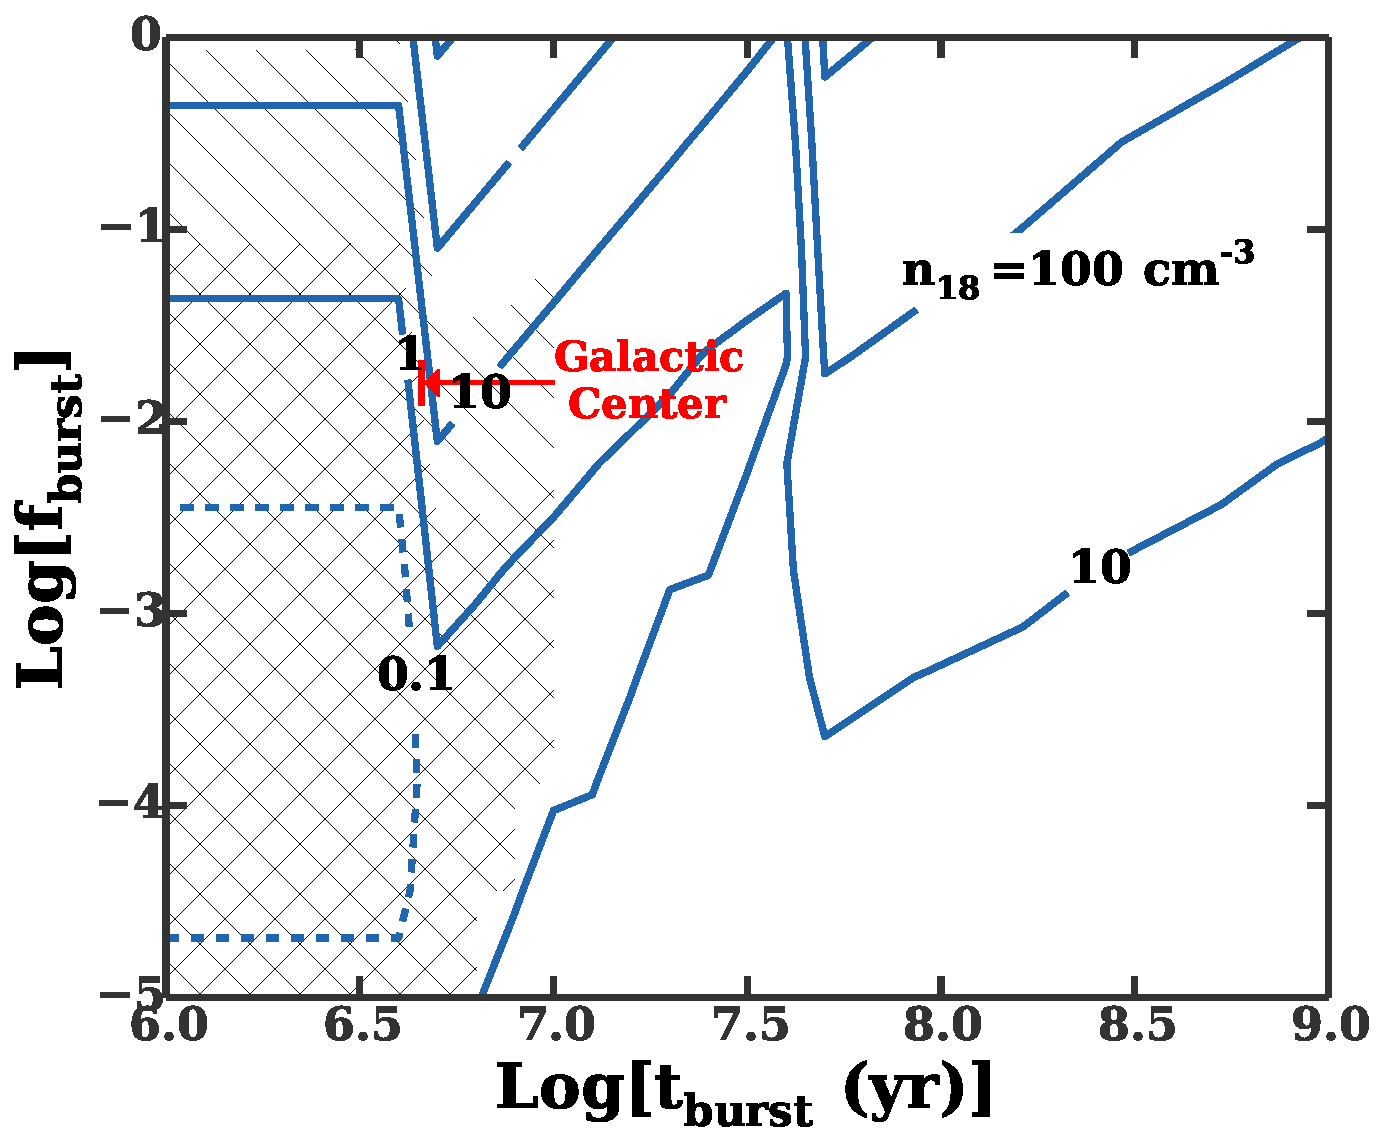
\includegraphics[width=8cm]{cnm_plot.pdf}
  \caption{\label{fig:param} Heating rates ($v_w$) and mass return
    parameters ($\eta$) for different star formation histories (gray
    lines). Solid, gray lines correspond to a star-burst of $<3$ Myr
    ago forming a fraction $f$ of the stars. The rest of the stars
    formed either a Hubble time ago (top line) or 1 Gyr ago (bottom
    line). The fraction $f$ increases and the gas density from left to
    right along these lines. The dashed, gray line corresponds to an
    alternate scenario in which there are two recent bursts in rapid
    succession in rapid succession: the older burst is $\sim 3$ Myr
    old (just at the point when stars are beginning to leave the main
    sequence). The contribution of this older burst increases towards
    the right, crossing boundary of the thermally unstable (``TI'')
    region below the thick black line. Iso-contours for the density at
    $10^{18}$ cm ($\mathrm{n_{18}}$) are shown as solid blue lines.} 
\end{figure}


\subsection{Empirical Constraints on CNM Density}

In this section we translate observed constraints on the accretion rate distribution of supermassive BHs into constraints on the CNM density.  The density $n$ at radius $r$ can be approximated from the inflow rate $\dot{M}$ as
\begin{equation}
\dot{M} = m \dot{M}_{\rm Edd}= f_{\rm in} 4 \pi r^2 \mu m_p n v,
\label{eq:mdot}
\end{equation}
where $n$ is the average density at radius $r$ and $f_{\rm in}$
represents the fraction of the large scale inflow, which actually
accretes onto the black hole.  If we assume that $r$ is interior to the sonic radius, then we can approximate $v$ as the free-fall velocity, $v_{\rm ff} = (GM_{\bullet}/2r)^{1/2}$.  In this case we obtain
\begin{equation}
n_{18} = 3 \times 10^3 M_{\bullet,7}^{1/2} m f_{\rm in}^{-1} {\rm
  cm}^{-3}
\label{eq:n18Edd}
\end{equation}
We expect that $f_{\rm in}$ could be quite small for highly sub
Eddington systems. For example, Faraday rotation measurements
\citep{Quataert+2000} show $f_{\rm in}\approx 10^{-3}$, in our own
galactic center. However, we expect $f_{\rm in}$ will be of order
unity for systems with $m\gsim 0.1$.  

\citet{Kauffmann+2009} present distributions of the OIII line
luminosity, ${\rm L[OIII]}/\Mbh$, for a range of BH masses ($10^7-10^{8.5}
\Msun$) from SDSS galaxies {\bf BDM fill in--AG what exactly?q}.  Assuming a bolometric correction, these
can be translated into distributions of Eddington ratio $m$.
According to \citet{Kauffmann+2009} ${\rm L[0III]}/\Mbh=1.7$, roughly
corresponds to Eddington ratio of 1. We adopt this conversion and
assume that the bolometric correction is independent of ${\rm
  L[0III]}/\Mbh$. {\bf AG--possibly factor of 2 discrepancy here to
  track down.}

The distribution of Eddington ratios for the lowest mass BH bin of $M_{\bullet} = 10^7 - 10^{7.25} \Msun$ (\citealt{Kauffmann+2009}; their Figure 4) is well fit by the expression,
\begin{align}
  F_{\rm cum}(m)=\frac{F_{m_0}}{2^{-1/s}}
  \left[\left(\frac{m}{m_0}\right)^{-a_1\,
      s}+\left(\frac{m}{m_0}\right)^{-a_2 \, s}\right]^{-1/s} \label{eq:khFit},
\end{align}
where $\{s, a_1, a_2, F_{m_0}\} =\{1.42, -0.166, -1.20, 0.235\}$.

\begin{figure}
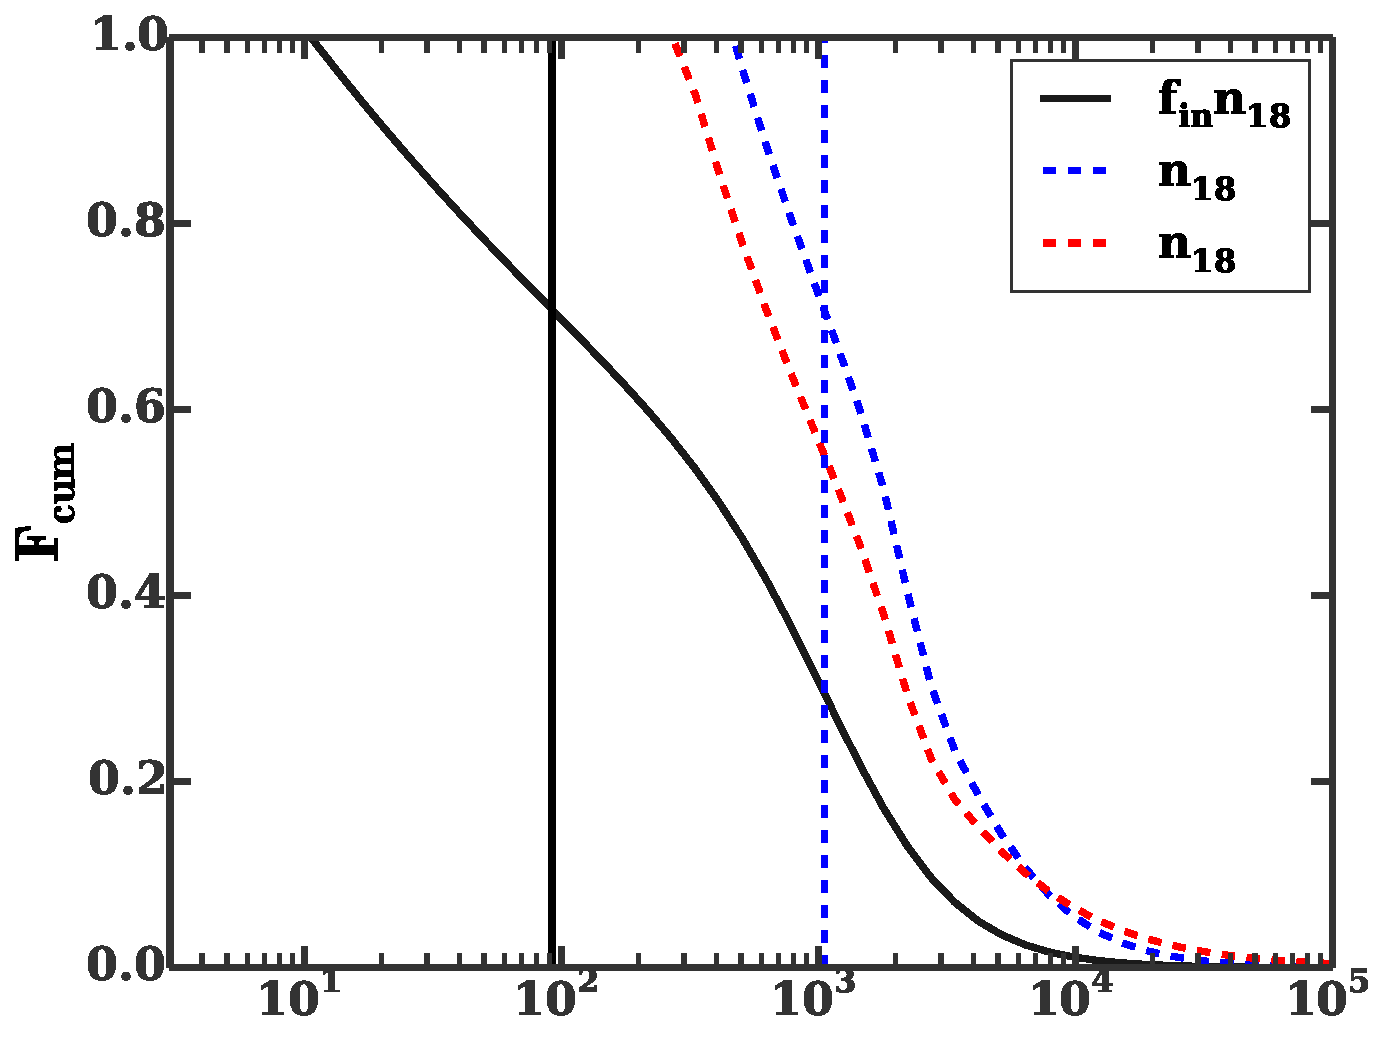
\includegraphics[width=8cm]{fcum_n18.pdf}
\caption{\label{fig:n18Cum} Fraction of black holes with $f_{\rm in}
  n_{18}$ greater than a given value--from equations~\eqref{eq:n18Edd}
  and~\eqref{eq:khFit}. Recall that $f_{\rm in}$ is the ratio of the
  true accretion rate onto the black hole to the inflow rate of
  free-falling gas at $10^{18}$ cm.   {\bf BDM: add vertical dashed line for eddington ratio of 1e-3}
% We expect $f_{\rm in}\approx
%   {10^{-3}-10^{-2}}$ for low densities and $f_{\rm in} n_{18} \simeq
%   1$ to be of order unity for $f_{\rm in} n_{18} \gsim 100 $.  In terms of
%   Eddington ratio, $m$, this corresponds to only a small fraction of
%   the large scale inflow reaching the hole for $m\lsim 0.01$, and an
%   order unity fraction reaching the hole for $m\gsim 0.01$.
}
\end{figure}


Fig.~\ref{fig:n18Cum} shows the distribution of $n_{18}$ resulting from combining this distribution with equation~\eqref{eq:n18Edd}.  The absence of galaxies with $f_{\rm in }n_{18} \lsim$ few cm$^{-3}$ places a lower bound on $n_{18}$ of a few cm$^{-3}$.  However, measurements of Eddington ratio below $\sim 10^{-3}$ are not reliable (shown with a vertical dashed line in Fig.~\ref{fig:n18Cum}), allowing a moderate fraction of galaxies ($\sim 20\%$) to have much lower gas densities.


In order to obtain the cumulative distribution for $n_{18}$, we need
a prescription for $f_{\rm in}$. We refer to \citet{Li+2013}, who
performed two-dimensional hydrodynamical simulations of axi-symmetric
rotating accretion flows. When the inflow rate on large scales was
very sub-Eddington ($\dot{M}/\dot{M}_{\rm Edd} \lsim 10^{-4}$),
cooling was inefficient and $f_{\rm in}$ was $\sim 0.01$. On the other
hand, when $\dot{M}/\dot{M}_{\rm Edd}\gsim 10^{-2}$, $f_{\rm in}$
approaches unity.  We use $\dot{M}_{\rm Acc}/\dot{M}_{\rm Bondi}$ in
their Figure 6 for $f_{\rm in}$.  With this choice only a third of
nuclei have $n_{18}>2,000$ and only 6\% have $n_{18}>10^{4}$ {\bf
  AG--TDEs could be subset which have very high or very low densities.}

Note that \citet{Li+2013} use an alpha viscosity prescription with
$\alpha=0.01$. We would expect that the value of $f_{\rm in}$ would be
sensitive to this choice. {\bf AG--a little more discussion of limitations.}

Two potential complications to keep in mind are (i) clumpiness of the
CNM and (ii) anistropy. The distributions above are
distributions of the {\it average} $n_{18}$.  Most likely, some of the
nuclear gas in a low density hot phase, while the rest is in high density
cold clumps/filaments. However, in this case the cold filaments would
be dissolved by the radiation from the jet...{\bf AG this needs
  justification/validation. If this is really true, then analytic
  section is faulty because it focuses on the hot phase.}

% {\bf AG Jeans criterion -- but be careful of tidal effects.}

AGN feedback would may blow low density bubbles in the
CNM. \citet{Russell+2013} used Chandra x-ray observations to measure gas
density and temperature profiles for a sample of massive elliptical
galaxies. The measured electron density on scales of $\sim 100
pc$ is $\gsim 0.1$ cm$^{-3}$. Note that the gas density at 100 pc
would be irrelevant for a TDE jet, but we would not expect the gas
density to be decreasing towards the galactic center in a steady
state. {\bf These are only massive ellipticals with $\Mbh\sim 10^{9} \Msun$.}

\subsection{Adopted gas density profiles}
 The following density provided a good fit to the CNM density profile
 of cusp galaxies.

\begin{align}
n=
\begin{cases}
  n_{18} \left(\frac{r}{10^{18} {\rm cm}}\right)^{-1} {\rm cm^{-3}} & r<r_b \\
  n(r_b) \left(\frac{r}{r_b}\right)^{-\beta} {\rm cm^{-3}} & r\geq
  r_b,\\
  \label{eq:profile}
\end{cases}
\end{align}

where $0.1 \Mbh[7]^{1/2} \lsim n_{\rm 18}\lsim 2,700
\Mbh[7]^{0.38} $ cm$^{-3}$.  

The gas density density experiences a break at radius $r_b$, the break
radius in the stellar density profile, where the stellar density
transitions from an inner power law slope $\delta_1\lsim 2$ to an outer
power law slope $\delta_2\gsim 2$. $r_b\gsim 100$ pc for cusp galaxies,
in which case the break radius may be safely ignored as it will be
well outside the jet deceleration radius. If there is a nuclear
star cluster present the effect $r_b$, the outer boundary of the
nuclear star cluster will correspond to a much smaller effective
$r_b\sim 1-5$ pc. However, even in this case the break radius is still
one too large scales to affect the light-curve evolution {\bf AG why?}
Thus, we don't include a break radius in our gas density profiles.

We perform simulations with CNM density $n=n_{18} \left(r/10^{18} {\rm
  cm}\right)^{-1}$ with $n_{18}$=2, 60, and 2000 to see what effect
varying the CNM density would have on the observed radio light-curve.

% The outer power law slope of the gas density will depend on the slope
% of the $\beta$ but will typically vary between 1.5 and 2. 

% We explore the parameter space of $n_{18}$, $\beta$, and $r_b$,
% adopting values for these parameters summarized by
% Table~\ref{tab:params} below


% \begin{table}
%   \caption{\label{tab:params} Summary of numerical parameters used for
%     the CNM profile (equation~\eqref{eq:profile}). A ``-'' in the $r_b$
%     or $\beta$ columns indicates that the gas density profile is a
%     single power law without any breaks. ``...'' in any column
%     indicates the entry is the same as the one above it.}
% \begin{minipage}{\columnwidth}
% \begin{tabular}{|l|l|l|}
% $n_{18}$ & $r_b [{\rm pc}]$ & $\beta$\\
% \hline
%   2     &  -    &  -\\
%   60    &  -    &  -\\
%   ...   &  1    &  1.5\\
%   ...   &  ...   &  2\\
%   2000  &  -    &  -\\
% \end{tabular}
% \end{minipage}
% \end{table}


{\bf AG cores...}

We also use a core galaxy profile to see how the shape of the stellar
density profile would affect the radio lightcurve. For core galaxies
the stellar density profile is not a pure power law. To simplify
things we will consider one particular slope for the stellar density
profile: $\rho_\star\sim r^{-\delta_1}$ with $\delta_1=1.1$. The gas
density profile may be approximated as

\begin{align}
\begin{cases}
n=n(r_s) k(x) & 0.4 \leq x\leq 2.0\\
n = 2.0 n(r_s) (x/0.4)^{-0.95} & x < 0.4\\
n = 0.75 n(r_s) (x/2.0)^{-0.26} & 2.0< x \leq r_s/r_b\\
n \sim x^{-1.5} & x>r_s/r_b\\
\end{cases}
\label{eq:cores}
\end{align}

Where, 

\begin{align}
  &x=r/r_s\\\nonumber
  &k(x)=\frac{45}{19} \frac{1}{x^{3/2}} \frac{1-x^{1.9}}{9-19
      x\frac{x^{0.9}-1}{x^{1.9}-1}}
\end{align}

To isolate the effects of the shape of the density profile, consider a
core density profile with $r_s=10^{18}$ cm, and $n_{18}=2000$: the
same as our high density cusp model.

% We consider a high density model (near the verge of thermal
% instability) and a low density model (near the lower limit of what
% stellar winds can give for the CNM density). The values $n(r_s)$ and
% $r_s$ are given in the table below. 

% \begin{table}
% \begin{tabular}{|l|l|l}
%  core models & $n(r_s)$ & $r_s$\\
% \hline
%  High & 2,500 $\Mbh[7]^{-0.32}$ cm$^{-3}$ &  4 $\times 10^{17}  
%  \Mbh[7]^{0.8}$ cm\\
%  Low & 0.1 $\Mbh[7]^{-0.24}$ cm$^{-3}$ & 6$\times 10^{16} \Mbh[7]$ cm
% \end{tabular}
% \end{table}

\section{TDE jets}
\label{sec:jet}

\subsection{Analytic Considerations}
\label{sec:analytic}


The mass of CNM swept up by the jet $2\pi\theta_{\rm j}^{2}\int m_p
n_{\rm cnm}(r) r^{2}dr$ equals its own rest mass $M_{\rm j} = E_{\rm
  j}/\Gamma_{\rm j}c^{2}$ at the characteristic (`Sedov') radius given
by 

\begin{equation}
r_{\rm sedov} = 8 \epsilon_{\rm
  j,-1}^{1/2} (\theta_j
\Gamma_j)^{-1}\Gamma_{10}^{1/2} n_{\rm 18}^{-1}\,{\rm pc}, 
\end{equation}

where we have taken $n_{\rm cnm} (r)=n_{18} \left(r/10^{18} {\rm
    cm}\right)^{-1}$, and $E_{\rm j}=0.1 \epsilon_{\rm j,-1} \Msun
c^2$.

From the continuity equation, the (co-moving) density of the jet is
given by (e.g. Uhm \& Beloborodov 2007)
 \begin{eqnarray}
   &n_{\rm j}& =  \frac{L_{\rm j}}{2\pi \theta_{\rm j}^{2}r^{2}\Gamma_{\rm j}^{2}c^{3}m_p(1 + r \dot{\Gamma_{\rm j}}/c\Gamma_{\rm j}^{3})} \approx  \frac{L_{\rm j}}{2\pi \theta_{\rm j}^{2}r^{2}\Gamma_{\rm j}^{2}c^{3}m_p}
\end{eqnarray}
%\approx \nonumber \\
%&&\left\{
%\begin{array}{lr}
%\frac{L_{\rm j}}{2\pi \theta_{\rm j}^{2} r^{2}\Gamma_{\rm j}^{2}c^{3}m_p}
%&  r \ll c\Gamma_{\rm j}^{2}t_{\rm j}\\
%\frac{L_{\rm j}t_{\rm j}}{2\pi \theta_{\rm j}^{2} r^{3}c^{2}m_p}
%,& r \gg  c\Gamma_{\rm j}^{2}t_{\rm j}\\
%\end{array}
%\right. 
%\label{eq:nj}
%\end{eqnarray}
where the second term in the denominator is generally negligible as
long as the Lorentz factor of the jet changes slowly
$\dot{\Gamma}_{\rm j} \ll c\Gamma_{\rm j}^{3}/r$, as can be shown to
be true at radii $r < r_{\rm sedov}$ as long as $\Gamma_{\rm j}$
changes on timescales $\gtrsim t_{\rm j}$.

A critical parameter is the ratio of the density of the jet to the CNM
\begin{eqnarray}
&&f \equiv \frac{n_{\rm j}}{n_{\rm cnm}}  \nonumber \\
&\approx & \left\{
\begin{array}{lr}
0.1\epsilon_{\rm j,-1}m_{\star}^{1/6}\Gamma_{10}^{-2}(M_{\bullet}/M_{\bullet, \rm Edd})^{-1}r_{\rm pc}^{-1/2}
&  M_{\bullet} < M_{\bullet, \rm Edd} \\
0.02\epsilon_{\rm j,-1}m_{\star}^{1/6}\Gamma_{10}^{-2}(M_{\bullet}/M_{\bullet, \rm Edd})^{-2/5}r_{\rm pc}^{-1/2}
,& M_{\bullet} > M_{\bullet, \rm Edd}\\
\end{array}
\right. 
\label{eq:f}
\end{eqnarray}
The blast wave of shocked matter expands with a common Lorentz factor $\Gamma_{\rm sh}$, which 
in the limit that $\Gamma_{\rm sh} \gg 1$ can be written (Sari \& Piran 1995; as can be derived from eq.~[\ref{eq:energy}] below)
\begin{eqnarray}
&&\Gamma_{\rm sh} \underset{\Gamma_{\rm sh} \gg 1}= \Gamma_{\rm ej}\left[1 + 2\Gamma_{\rm ej}f^{-1/2}\right]^{-1/2} \underset{f \ll 4\Gamma_{\rm j}^{2}}\approx 0.71\Gamma_{\rm ej}^{1/2}f^{1/4} \approx \nonumber \\
&&\left\{
\begin{array}{lr}
1.26\epsilon_{\rm j,-1}^{1/4}m_{\star}^{1/24}(M_{\bullet}/M_{\bullet, \rm Edd})^{-1/4}r_{\rm pc}^{-1/8}
&  M_{\bullet} < M_{\bullet, \rm Edd} \\
0.84\epsilon_{\rm j,-1}m_{\star}^{1/24}(M_{\bullet}/M_{\bullet, \rm Edd})^{-1/10}r_{\rm pc}^{-1/8}
,& M_{\bullet} > M_{\bullet, \rm Edd}\\
\end{array}
\right. 
\label{eq:gammash}
\end{eqnarray}
We thus conclude that the shocked material will be decelerated to
mildly relativistic velocities on scales $r \sim r_{\rm sedov}$.  Note
the $\Gamma_{\rm j}$ cancellation.  For Sw J1644+57, the inferred BH
mass was $\lesssim 1/30M_{\bullet,\rm Edd}$ and $\epsilon_{\rm j,-1}
\sim 0.1-1$, implying $\Gamma_{\rm sh} \sim $ few on scales $\sim 0.3$
pc.

In the above we have assumed that the jet expands freely.  According
to Bromberg et al.~(2011), a jet of intrinsic opening angle
$\theta_{\rm j}$ will be self-collimated if its luminosity is less
than a critical value

\begin{equation}
L_{\rm j} < L_{\rm crit} = 2\pi \theta_{\rm j}^{2}n_{\rm cnm} m_p c^{3}\theta_0^{-4/3},
\end{equation}

i.e.~ if

\begin{equation}
f < 0.2(\theta_{\rm j}/0.1)^{2/3}(\theta_{\rm j}\Gamma_{\rm j})^{-2}
\end{equation}

According to equation (\ref{eq:f}) this condition is achieved at a radius 
\begin{eqnarray}
r_{\rm sc}  &\approx & \left\{
\begin{array}{lr}
0.25\epsilon_{\rm j,-1}^{2}m_{\star}^{1/3}(\theta_{\rm j}/0.1)^{8/3}(M_{\bullet}/M_{\bullet, \rm Edd})^{-2}{\rm pc}
&  M_{\bullet} < M_{\bullet, \rm Edd} \\
0.01\epsilon_{\rm j,-1}^{2}m_{\star}^{1/3}(\theta_{\rm j}/0.1)^{8/3}(M_{\bullet}/M_{\bullet, \rm Edd})^{-4/5}{\rm pc}
,& M_{\bullet} > M_{\bullet, \rm Edd}\\
\end{array}
\right. 
\label{eq:rsc}
\end{eqnarray}


\subsection{Jet Models}
\label{sec:numerical}

The jet-CNM interaction is simulated using one and two-dimensions, and
the resulting synchrotron emission is computed using the same
procedure described in \citet{Mimica+2015}. We assume the same angular
Lorentz factor dependence as in previous paper (i.e., $\Gamma = 10$
for the fast inner core and $\Gamma = 2$ for the slow outer sheath),
but we introduce a number of modifications regarding the jet energy
when performing 1D simulations.

\subsection{1-d vs. 2-d Models}
\label{sec:2d}

The preferred numerical model for Swift J1644+57 \citep[Fig.10
in][]{Mimica+2015} was obtained using 2D simulations (the red line in
that figure). However, the light curve of a 1D version of the same
model \citep[black line in Fig. 10 in][see also section 4.2 of that
paper]{Mimica+2015} matches the 2D light curve only at early times,
when the emission from the inner relativistic jet dominates, while at
late times, when the emission from the slow outer core dominates, the
1D model overestimates the emission from the 2D model. In this work we
found a modification of the 1D model that alloed its light curves to
match the 2D results much more closely.

We first summarize the two-component model as presented in
\citet{Mimica+2015}. We assume that the fast inner core spans an
angular interval $[0, 0.1\ {\rm rad}]$, while the slow outer sheath
occupies $[0.1\ {\rm rad}, 0.5\ {\rm rad}]$. For both components we
assume $E_{\rm ISO} = 4\times 10^{54}$ erg. The crucial thing to
notice is that, keeping $E_{\rm ISO}$ constant, the true jet energy
depends only on the angular interval: $E_{\rm jet} = E_{\rm ISO}
(\cos\theta_{\rm j,min} - \cos\theta_{\rm j,max})$. Note that the
hydrodynamic evolution of the components is independent of angle in 1D
simulations, but the radiative transfer/light-curve calculation is
sensitive to the jet geometry.

Second, we note that, although the sheath is injected in a relatively
narrow angular interval, at late stages of the jet evolution the bow
shock created by its ineraction with CNM spans a much larger interval,
i.e. the slow component becomes almost isotropic \citep[bottom two
panels in Fig. 8 in][]{Mimica+2015}. This is the reason for the
discrepancy with the 1D simulation, because there the slow component
angular size is fixed to the initial one. We note that the stage at
which the jet becomes ``isotropic'' depends on the CNM density,
i.e. the denser the CNM, the faster this is expected to happen ({\bf
  PM: references? Zhang \& MacFadyen or de Colle \& Ramirez-Ruiz? need
  to check later}).

Since the agrrement between 1D and 2D models is good at the early times (when the fast component dominates), we modify only the slow component in 1D models. We assume that is spans $[0.1\ {\rm rad}, \pi/2\ {\rm rad}]$ and lower its $E_{\rm ISO}$ so that the true jet energy remains unchanged with respect to the original model:
\begin{equation}\label{eq:Eiso}
 E_{\rm ISO, new} = E_{\rm ISO} \left(\frac{\cos(0.1) - \cos(0.5)}{\cos(0.1) - \cos(\pi/2)}\right)\approx 0.12 E_{\rm ISO}\, .
\end{equation}

We assume $E_{\rm ISO} = 4\times 10^{54}$ erg, and that the jet luminosity time dependence is the same as in \citet{Mimica+2015},
\begin{equation}\label{eq:lum}
L_j(t) = L_{j,0}\max\left[1, (t/t_0)\right]^{-5/3}
\end{equation}
where $t_0 = 5\times 10^5$ seconds and $L_{j, 0}$ can be determined from $E_{\rm ISO}$ by integrating equation~\ref{eq:lum} in time from $0$ to $\infty$. We show a comparison of this modified 1-d approach with the true 2-d result in Figure~\ref{fig:1d2dB}, for $n_{18}=60$ and $n_{18}=2000$.

\begin{figure*}
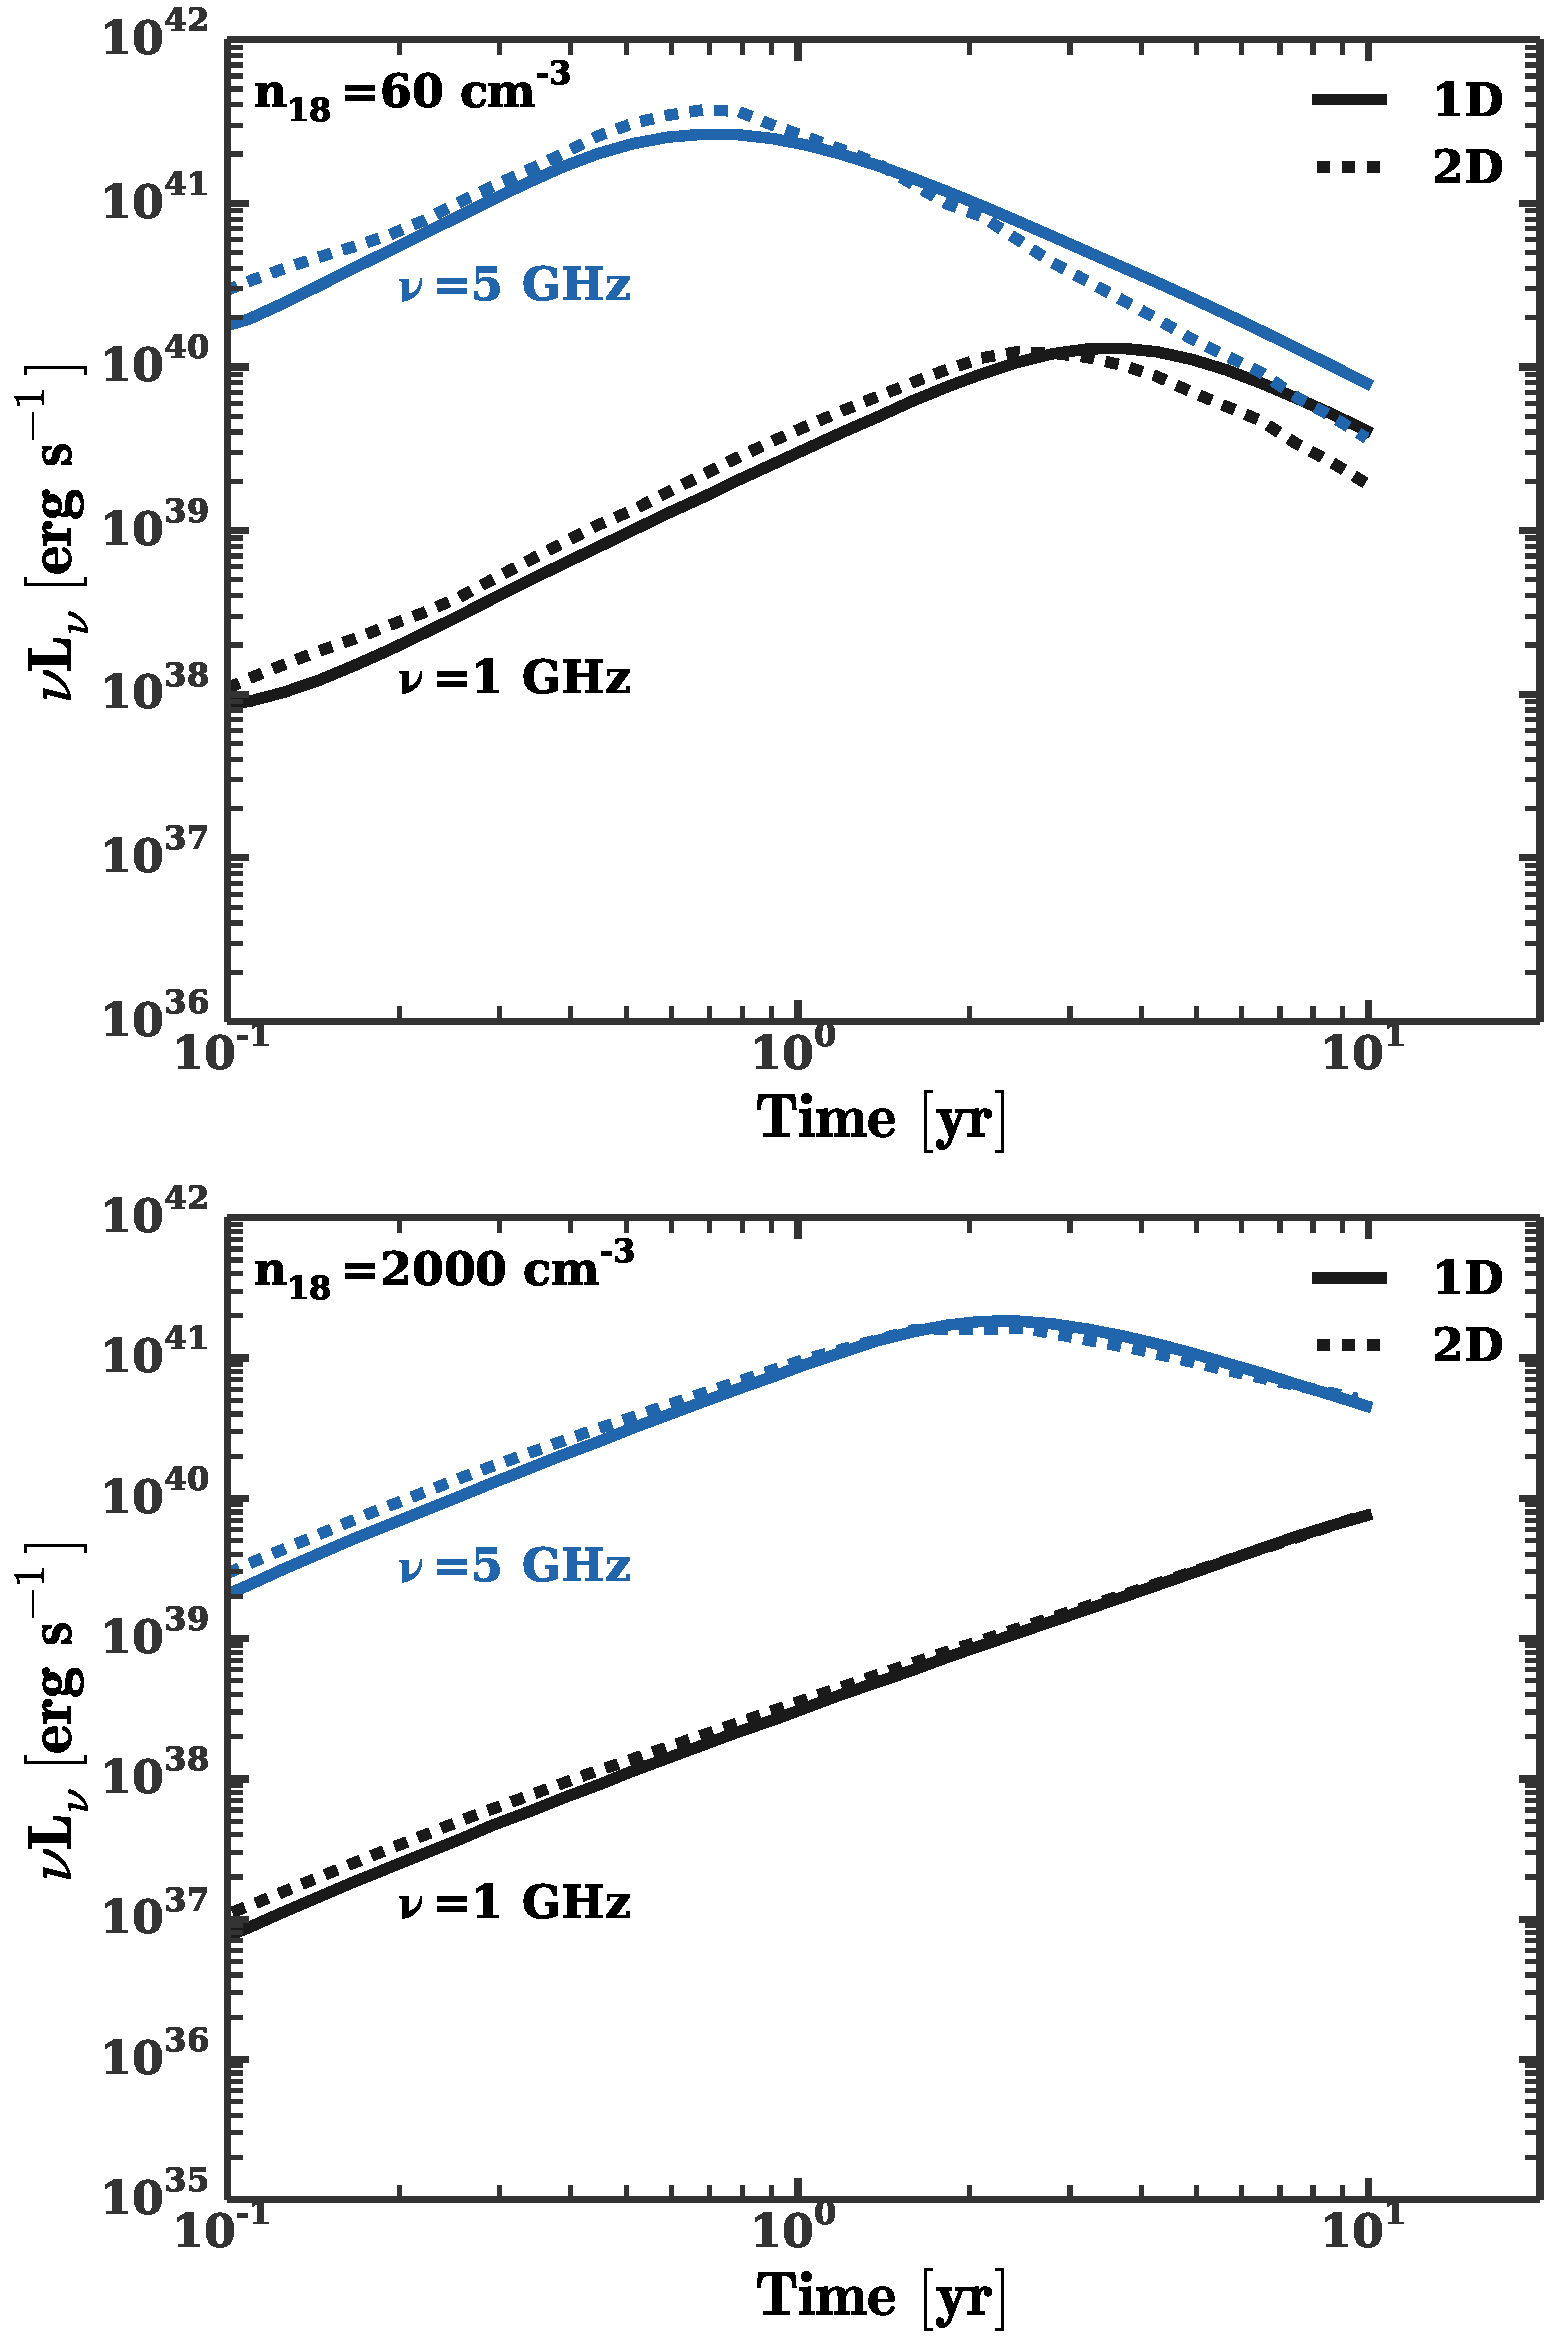
\includegraphics[width=16cm]{1d_2d.pdf}
\caption{\label{fig:1d2dB} Comparison light-curves for $n_{18}=60$
  (top) and $n_{18}=2000$ (bottom) for frequencies of 1 GHz (left) and
  30 GHz (right) and an observer angle of 0.8 radians to the jet
  axis. We assume an $n\sim r^{-1}$ density profile for $n_{18}=2000$,
  but take $n\sim r^{-1.5}$ for $n_{18}=60$ for computational
  convenience.}
\end{figure*}


\section{Results}
\label{sec:results}

\subsection{Effects of gas density}

In Fig.~\ref{fig:upper_limits} we show the on-axis light curves for
our fiducial jet model and CNM density profile $n=n_{18} (r/10^{18}
{\rm} cm)^{-1}$ cm$^{-3}$ with $n_{18}$=2, 60, and 2000 cm$^{-3}$. The
higher density models peak at later times with smaller peak
luminosities {\bf AG Do we understand this? Is this due to the effect
  of self-absorption?}

{\bf AG it would probably be good to have a figure showing the
  different components contributing to the emission.} The radio light
curve has contributions from both the slow and fast jet
components. The fast component dominates at
early times for the $n_{18}=2$ and 60 lightcurves, while the slow
component dominates for all times as frequencies for
$n_{18}$=2000. Generally, the fast component is more important at
higher frequencies, and lower densities.

We also show radio upper limits and detections for various TDE
candidates in Fig.~\ref{fig:upper_limits} (these were compiled from
various sources into Table 1 of \citealt{Mimica+2015}). Overall, the
measurements were taken too late to be strongly constraining,
especially for the low density models: the lightcurves or $n_{18}=2$
peak on time-scales of months, while many of the radio measurements
were taken decades after the TDE flare.

\begin{figure} 
  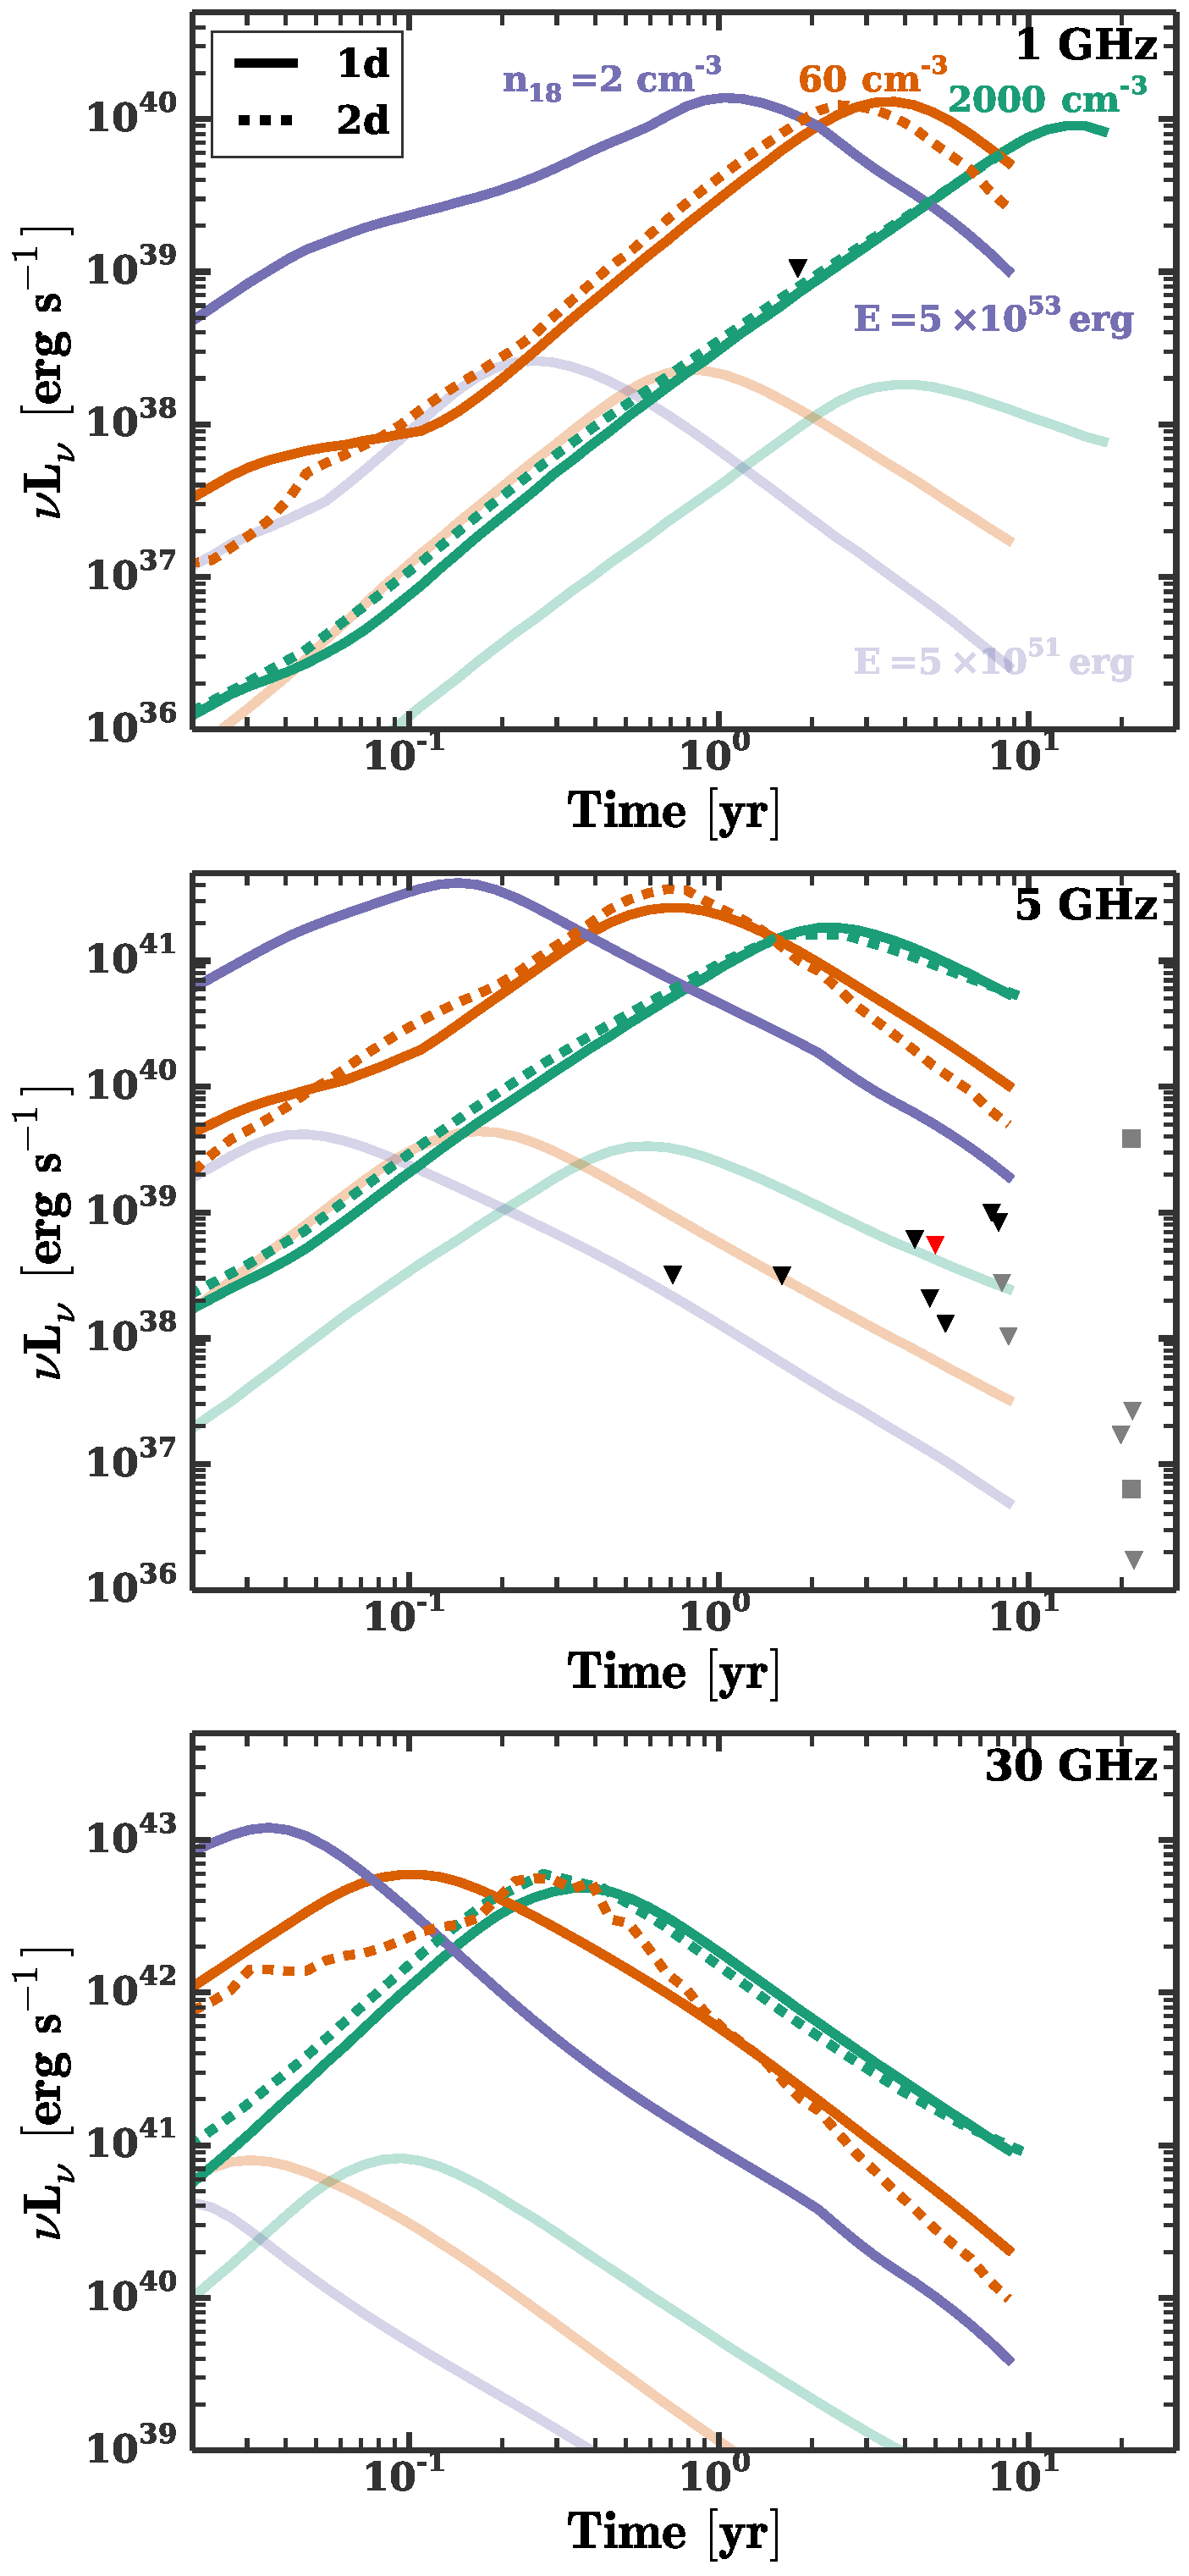
\includegraphics[width=8cm]{lightcurves.pdf}
  \caption{\label{fig:upper_limits} On-axis radio light-curves for
    fiducial jet model and CNM density profile $n=n_{18} (r/10^{18}
    {\rm cm})^{-1}$, for three different values of n$_{18}$: 2, 60,
    and 2000. Radio upper limits and detections are shown as
    black/gray triangles and squares respectively (compiled in Table 1
    of \citealt{Mimica+2015}). The single upper limit in the top panel
    corresponds to 1.4 GHz. Gray triangles and squares in the middle
    panel indicate upper limits and detections at 3.0 GHz, while black
    triangles indicate upper limits at 5.0 GHz.}
\end{figure}

\subsection{Effect of gas density profile}
We have also computed the radio light-curves for different shapes of
the gas density profile, while holding $n_{18}$ fixed. We compute the
results for $n_{18}=2000$ for both our fiducial $n\sim r^{-1}$ profile and
the core galaxy profile, shown in equation~\eqref{eq:cores}. The
former would more relevant for a cuspy stellar density profile with
stellar density $\rho_{\star}\sim r^{-2}$, while the latter would be more
appropriate for a flatter $\rho_{\star}\sim r^{-1}$ stellar density
profile. As a steeper stellar density is more favorable for producing
tidal disruption events, we would expect most events to occur is cusp
rather than core galaxies.

The results are virtually indistinguishable as shown in
Fig.~\ref{fig:cores}. Overall, the late time evolution of the
light-curve is insensitive to the slope of the stellar density profile
(see Figure 3 of \citealt{Mimica+2015}) {\bf AG this is only for the
  fast narrow component--how do we justify this more generally?}.


\begin{figure} 
  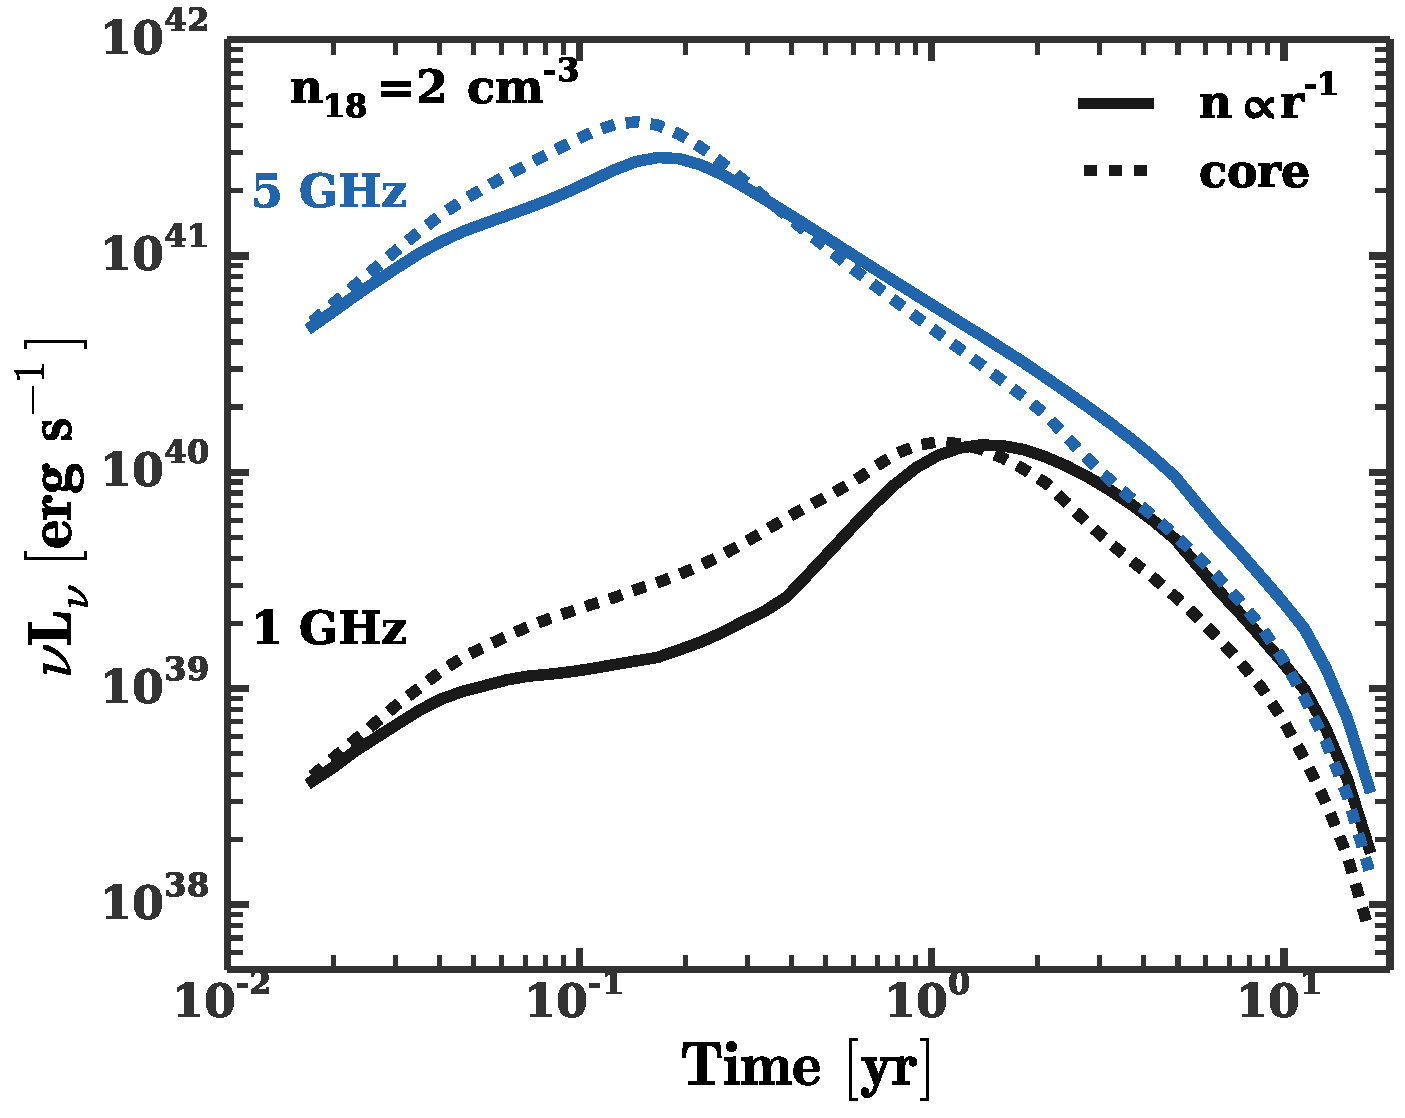
\includegraphics[width=8cm]{fig_cores.pdf}
  \caption{\label{fig:cores} Comparison of the light-curves for
    $n_{18}=2000$ and two different CNM gas density profiles: $n\sim
    r^{-1}$ and the core galaxy profile from \eqref{eq:cores} with
    $r_s=10^{18}$ cm and $n(r_s)=2000$, so that we can isolate the
    effect of the shape of the density profile. 4 pi correction}
\end{figure}


\subsection{Effects of viewing angle}


\section{Discussion}
\label{sec:disc}
{\bf AG -- Observational prescriptions and rates?}

\section{Summary and Conclusions}
\label{sec:conc}

\clearpage
  \footnotesize{
    \bibliographystyle{mnras}
    \bibliography{master}
  }

\end{document}
